\chapter{Introduction}
\label{ch:Introduction}
\section{The structural design process}
Before a new structure can be built, it must be designed. This design phase, here termed the \textit{structural design phase}, is a very important step in the building process. The total cost of the structure and its energy performance and structural performance are largely dependent on the structural design process \cite{Mueller2014}. 

The structural design process is rarely straightforward. Rather, solutions are reached through an iterative and often chaotic process. This process can be divided into the following four steps \cite{schlaich2006challenges}:

\begin{enumerate}  
\item \textbf{Conception}: The most important design step, where the overall design concept and significant details are developed.
\item \textbf{Modeling}: Idealization and simplification of the structural design concept, building of models for structural analysis, and calculation of forces.
\item \textbf{Dimensioning}: Determining sectional dimensions of structural members depending on the choice of materials.
\item \textbf{Detailing}: Final details of nodes and connections, including the creation of construction documents.
\end{enumerate}

In reality, there is no clear distinction between the different design steps, and the process can iteratively move back and forth until a solution is reached. In this thesis, the term ``conceptual design’’ refers to the first design step of conception and the initial phase of the modeling step. In the initial design phase, there is considerable design freedom. At the same time, the impact on the final result of the decisions taken at this early stage is often crucial. In contrast, both the design knowledge and the availability of design tools increases as the design matures \cite{schlaich2006challenges} \cite{Hsu2000}; see Figures \ref{fig:freedom-vs-knowledge} and \ref{fig:impact-tools}. The design knowledge comprises all that is known of the final design, from the color of the facade to the dimensions of structural members. The lack of tools for the initial design phase, combined with the high impact of decisions, creates the opportunity to develop tools that support designers in making well-informed decisions in the conceptual design phase.

\begin{figure}
  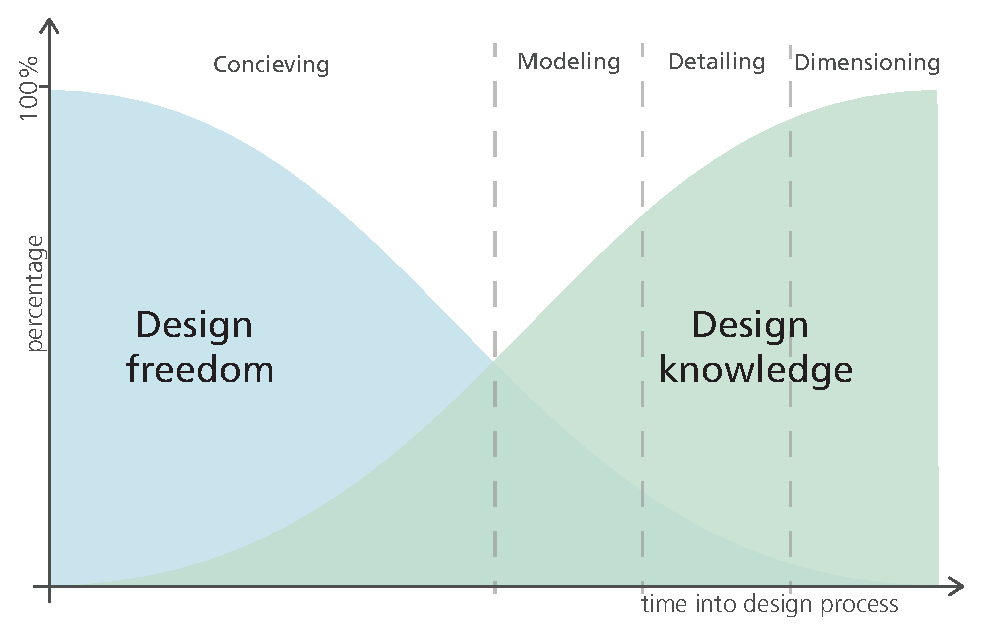
\includegraphics[width=350pt]{graphics/freedom-vs-knowledge.eps}
  \caption{Structural design process \cite{Mueller2014}}
  \label{fig:freedom-vs-knowledge}
\end{figure}

\section{Problem statement}
Many different geometric modeling tools are currently available to architects. These geometric modeling tools have, since their introduction in the 1980s, grown increasingly sophisticated. They have also, together with the widespread perception of the benefits of technological innovation, created a more intimate relationship between technology and design. This relationship has resulted in parametric design and scripting methods that can generate complex shapes and forms \cite{sakamoto2008control}. The distinct separation found in practice, whereby architects use geometric modeling tools and engineers use analysis tools, further reinforces the roles of the architect as \textit{form-giver} and the engineer as \textit{form-verifier} \cite{mueller2013integrated}. To move away from this separation, this thesis uses the term \textit{designer} to represent either an engineer or an architect. Instead of the current practice, it would be beneficial if engineers and architects collaborated as designers in the structural design process. This would allow physical demands (e.g., structural performance, construction costs, operational energy needs, acoustics) to work as an inspiration, rather than as a constraint on what is possible, in finding new, high-performing geometric forms. 
In the current practice, the architect often conceives a design without any involvement from the structural engineer. Hence, the importance of the conceptual design phase is often overlooked, and structural aspects are sometimes only considered in the later design stage \cite{schlaich2006challenges}. A contributing factor to this is that very few computational tools are available for conceptual design. 

\begin{figure}
  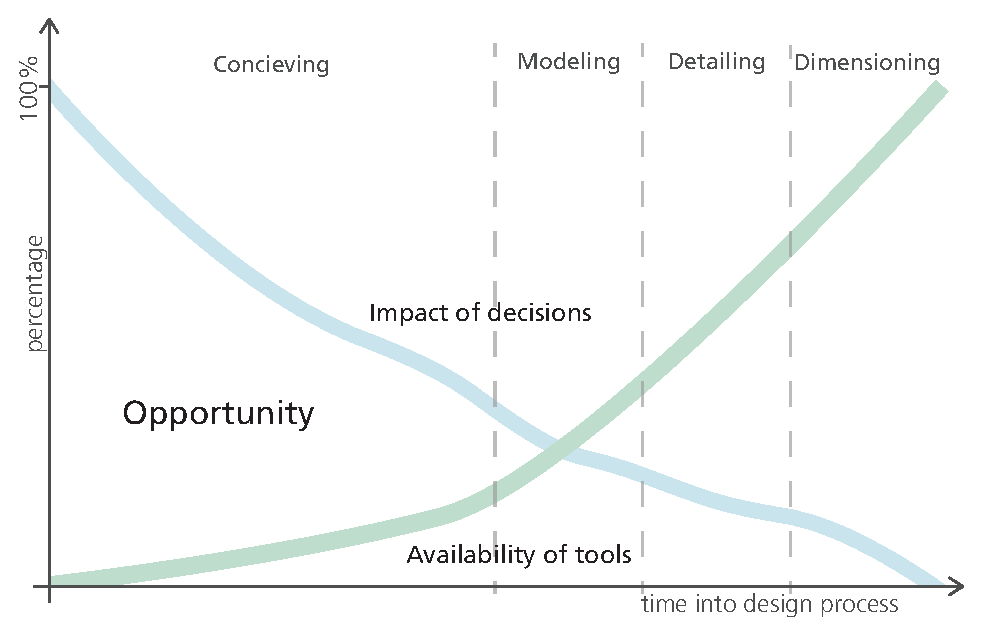
\includegraphics[width=350pt]{graphics/impact-tools.eps}
  \caption{Impact of decisions and availability of tools in the design process \cite{Hsu2000}}
  \label{fig:impact-tools}
\end{figure}


In developing such computational tools, the challenge lies within the fuzzy nature of the problem, as the knowledge and constraints of the problem are often imprecise and incomplete \cite{Hsu2000}.

Conventional advanced structural analysis software requires precise knowledge of the problem, and is insufficiently agile to follow a designer’s iterative workflow. Conventional structural analysis software has been developed for use in the late design stage, after the major design decisions have been made, for the engineer to verify the form. 

A subsequent problem with the traditional workflow in which the architect is the form-giver and the engineer is the form-verifier arises from the availability of a very detailed geometric model. It can be tempting for the engineer to directly perform a full analysis on the detailed geometry, something that is possible with current structural analysis software. Instead, if the engineer starts with a simple mathematical model and then gradually increases the complexity (known as hierarchical modeling, see Figure \ref{fig:hiarchical-modelling}), the risk of fatal mistakes decreases \cite{Bathe2006}. 

By starting with a simple mathematical model, the engineer can focus on, and gain a better understanding of, the overall structural behavior, such as how stresses propagate through the structure, the magnitude of the stresses in different structural members, and so on. This information is valuable in confirming the feasibility of the results given by more advanced mathematical models. It has been shown that the premature use of advanced structural analysis software has a negative effect on the conceptual understanding and quality of the design \cite{Froderberg2014}.

In the present work, two similar conceptual design tools have been developed. The two applications make use of simple mathematical models, thus enabling structural modeling to be used earlier in the structural design process. The motivation for this is two-fold. First, it provides designers with valuable feedback on structural performance in the conception phase, when the impact of decisions is high. Second, it presents engineers with valuable feedback on structural behavior before a more advanced model is used. 

\begin{figure}
  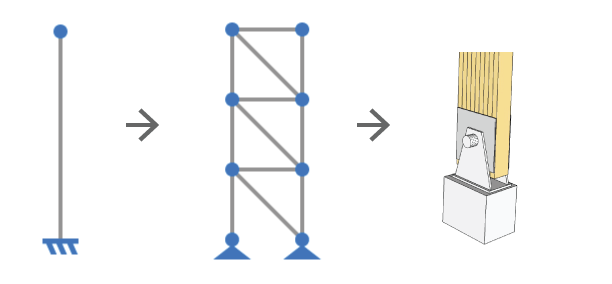
\includegraphics[width=270pt]{graphics/hiarchical-modelling.png}
  \caption{Hierarchical modeling}
  \label{fig:hiarchical-modelling}
\end{figure}

The type of design tool used to generate and represent ideas also affects the quality and quantity of early prototypes. It has been shown \cite{Haggman2015} that physical prototyping generates a higher quantity of prototypes per unit time than using CAD or conventional sketching. The prototypes developed using physical prototyping were also perceived to be more novel than the other prototypes. However, the prototypes that were perceived as more novel also tended to fare poorly on all other measurable qualities \cite{Haggman2015}. 

In the present work, the prototypes are structural models. As computational models are used, measurable performance indices can be computed and presented to users in real time. This has the potential to improve the quality of the structural models. The measurable performance and guidance in the present work focuses on the geometrical form of the structure, as this has the greatest potential to improve the structural performance \cite{Mueller2014}. 

\subsection{Examples of well-executed conceptual structural design}
As mentioned earlier, structural demands can be integrated earlier in the design process by using them as the inspiration for geometric forms, instead of constraints on what is possible. Integrating structural demands earlier in the design process has, amongst other, the potential to reduce the amount of material needed, thus reducing the environmental impact and costs of the project as a whole. 

\begin{figure}
  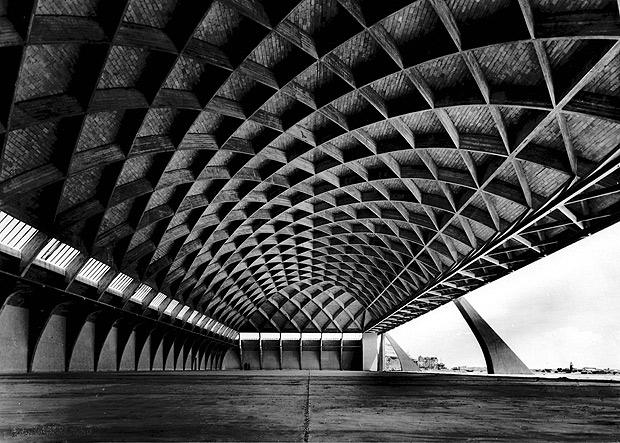
\includegraphics[width=350pt]{graphics/nervi.jpg}
  \caption{Pierre Luigi Nervi - Air hangar, built 1936}
  \label{fig:nervi}
\end{figure}

Good examples of well-executed conceptual designs include the structures designed by the Italian architect-engineer Pierre Luigi Nervi (see example in Figure \ref{fig:nervi}). Despite the complexity of the structures, his designs were often selected because they required less material than those of his competitors, and were therefore the cheapest to build \cite{Addis2007}. This type of complex concrete structure is unfeasible when labor costs are high, because of the extensive formwork required \cite{Todisco2015}. However, this could of course change in the future with the emergence of robots and digital manufacturing \cite{MadeByRobots}.

\textit{``His buildings are most remarkable for the clarity of their engineering. The power and grace of these extraordinary shapes and patterns stems directly from their structural logic, and are inseparable from it''} – Ada Louise, talking about Pierre Luigi Nervi, 1960 \cite{Mueller2014}

The Shenzhen CITIC Financial Center (see Figure \ref{fig:Shenzen}) is a more recent example of well-executed integrated conceptual design. The perimeter frames are inspired by research on optimal discrete truss geometries to minimize the material needed \cite{Stromberg2012a}.

\begin{figure}
  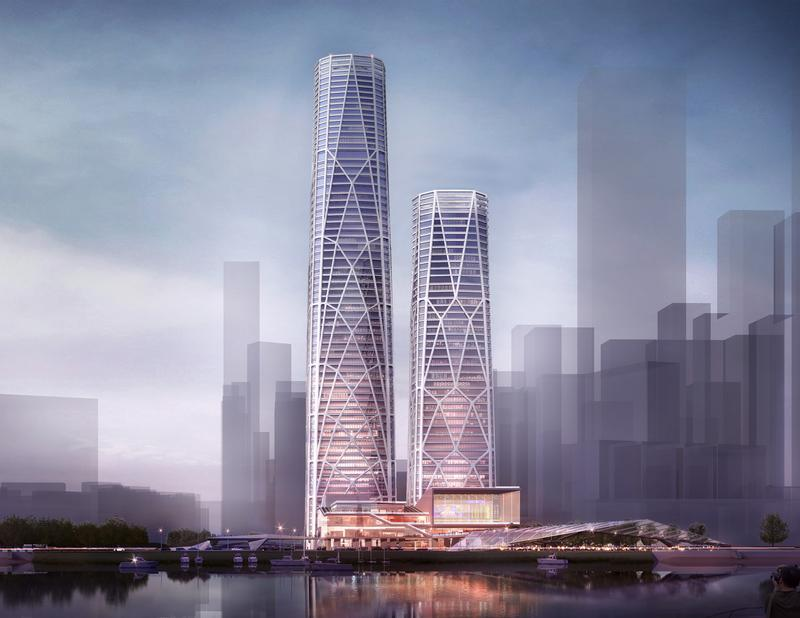
\includegraphics[width=350pt]{graphics/shenzen.jpg}
  \caption{Shenzen CITIC Financial Center, Lead Architectural Partner: Craig W. Hartman, Lead Structural Partner: Mark Sarkisian.  Rendering © Skidmore, Owings \& Merrill LLP, 2016}
  \label{fig:Shenzen}
\end{figure}

Designing Nervi’s air hangar in 1936 required a very thorough understanding of structural mechanics. At the time, Nervi was one of very few engineers that were capable of successfully designing such a structure. The CITIC Financial Center was also designed by a team of distinguished designers. The difference between the two examples is that the latter used computer simulations in the design process. 

\subsection{Computational design tools}
Computational design tools have the ability to make computer simulations readily available in the design process, thus helping to guide the designer towards solutions that perform well. Various tools have been developed for this purpose, and a review of existing tools and the methods that they implement is given in \ref{ch:Computational methods}. Unlike conventional structural analysis software, these tools were developed to follow the designer’s iterative workflow. 

Allowing these computational tools to follow the designer’s iterative workflow places high demands on their user interfaces. Most existing computational design tools were developed for mouse and keyboard input. In the present study, alternative input devices that allow for more direct input are explored. 

\section{Research methodology }
\subsection{Aim of research}
The long-term goal of this research is to improve the conceptual design phase by integrating structural demands early in the design process. An improved conceptual design phase has the potential to improve certain qualities of structures in the built environment. These qualities include the structural performance, construction costs, operational energy needs, and acoustics.

The specific aims of the present work are:
\begin{itemize}  
\item  To create intuitive conceptual structural design tools that allow users to easily explore different design alternatives.
\item To improve the human--computer interaction for such tools through the use of new, novel user input devices. 
\end{itemize}


\subsection{Research questions}
\begin{itemize}  
\item How can human--computer interaction be improved in conceptual structural design tools?
\item  Which computational methods can be used to improve the conceptual design phase? 
\end{itemize}

\subsection{Research approach and limitations}
The present research is a multi-disciplinary study involving structural mechanics, computer science, and architecture. Methods from structural mechanics are used to provide the user with guidance and feedback. The development of user interfaces and use of programming techniques is an area of computer science, and studying conceptual design and finding geometrical forms is a branch of architecture. Any successful tools developed in this research could potentially be used in practice.

Different research approaches can be used to investigate how to improve the conceptual structural design phase. This study only investigates how new computational tools can enhance the conceptual design phase. Project management, social aspects, and culture are not considered in this work.

Many different computational methods have been used for conceptual structural design. Some promising methods are discussed in Chapter \ref{ch:Computational methods}, and a selection of these methods are used in the present work.

\subsection{Outline}
\textbf{Part I} gives an introduction to the research area and reviews the literature in this field. This part is similar to, but an extension of, the introductory sections in the appended papers. \textbf{Chapter \ref{ch:Introduction}} provides an introduction to the research area, and explains the motivation and importance of this work. \textbf{Chapter \ref{ch:Human-computer interaction}} introduces the concept of human--computer interaction and describes state-of-the-art technologies such as new input devices. \textbf{Chapter \ref{ch:Computational methods}} presents computational methods that can be applied to conceptual design. Different optimization methods, particularly genetic algorithms, are discussed, as these methods will be used in future work. \textbf{Chapter \ref{ch:Literature review}} reviews existing conceptual structural design tools. In \textbf{Chapter \ref{ch:Integrating structural feedback}}, the requirements for integrating structural feedback in the conceptual design are presented, and the present work is summarized. The publications that have resulted from this work are listed in \textbf{Chapter \ref{ch:Summary of appended papers}}, and \textbf{Chapter \ref{ch:Results discussion}} summarizes the intellectual contributions of this study. \textbf{Part II}  contains the appended publications.

